\documentclass[12pt , a4paper]{article}
\usepackage{fullpage}
\usepackage{float}
\usepackage{amsmath,amssymb,amsfonts}
\usepackage{graphicx}
\usepackage{float}
\usepackage{csvsimple}
\usepackage[utf8]{inputenc}
\usepackage{amsmath}
\title{My First Latex Document}
\author{Sahil Deshpande}
\date{November 26, 2022}
\begin{document}

\begin{Huge}
\begin{center}
\bf Assignment 1
\end{center}
\end{Huge}
\maketitle
Hi! This is Sahil Deshpande, and I am really excited to show my first latex document!

\section*{Overview}
LaTeX is a document preparation system for high-quality typesetting. It is most often used for medium-to-large technical or scientific documents but it can be used for almost any form of publishing.
\section*{Text Editors}
\subsection*{E – TextEditor}
E – TextEditor download page E – TextEditor, or just called E, is TextMate for Windows. It has a host of useful features that developers will appreciate, such as a personal revision control system to ease the burden of managing multiple versions of a file, ultimate customization possibilities, and a collection of automated tasks to save you time and improve your productivity. Check out the Keyboard Shortcuts Cheatsheet to make writing with E more efficient.
\subsection*{TextPad}
TextPad download page TextPad is a general purpose text editor for Windows-based systems. It has plenty of features like a spell checker for 10 languages, a Warm Start feature which lets you start the program from where you left off when you last opened it, and a keystroke macro recorder for automating keystrokes (which can save you a ton of time from typing frequently-used code), and lots more.

\pagebreak

\begin{Huge}
\begin{center}
\bf Assignment 2
\end{center}
\end{Huge}


\pagebreak

\begin{center}

\Large \textbf {COEP Technological University}
\vspace{0.5cm}

\large \textbf {Department of Mathematics} 
\vspace{0.5cm}

\large \textbf {Test 1 Examination}\\
\end{center}
\noindent MIS : 
\begin{tabular}{|c|c|c|c|c|c|c|c|c|}
\hline
 &  &  &  &  &  &   &  &  \\ \hline
\end{tabular}\\
\rule{\textwidth}{0.1pt}\\


\begin{large}
\noindent \textbf {Instructions : }
\end{large}
\begin{itemize}
\item All questions are compulsory.
\item Writing anything on the question paper is not allowed.
\item Mobile phone and programming calculators are strictly prohibited.
\item Exchange/Sharing of stationary, calculator etc. is not allowed.
\item Each question of Section A carries 4 marks each.
\item Each question of Section B carries 3 marks each.
\end{itemize}
\rule{\textwidth}{0.1pt}
\section*{Section A : Calculus}

\begin{enumerate}
\item Solve the following differential equation :          
\begin{align*}
3x(xy - 2)\,dx +(x^3+2y)\,dy=0 
\end{align*}
\item Solve the following differential equation using method of undetermined coefficients
\begin{equation*}
x^3y''' + x^25y'' + 2xy' + 5y = x^2\sin x
\end{equation*}
\item Find the set of critical points and determine the absolute maximum and minimum
values of each function on the given interval.
	\begin{enumerate}
	\item $ \displaystyle{f(x)=\frac{-1}{x+3}}\,\, , \,-2\leq x \leq 3 $
	\item $ |x|x-x \,\, ,\, x \in \mathrm{R} $
	\item $ \displaystyle f(x)=\sqrt{4-x^2} \, \, ,\, -\sqrt{2}\leq x \leq 1 $
	\item $ \displaystyle f(\theta)= \sin \theta \,\, ,\, \frac{-\pi}{2} \leq \theta \leq \frac{5\pi}{6} $
	\end{enumerate}
\item Prove the following inequality :
\begin{equation*}
\frac{b-a}{\sqrt{1-a^2}} < \sin ^{-1} b - \sin ^{-1} a < \frac{b-a}{\sqrt{1-b^2}}\,\,\,\,\,\, \mathrm{for} \,\, 0 < a < 1\,\,\, \mathrm{and}\,\,\, 0 < b < 1
\end{equation*}

\newpage
\item Prove the following :
\begin{equation*}
\displaystyle \beta (p,q) = \int_0^\infty \frac{y^{q-1}}{(1+y)^{p+q}}\,dy = \int_0^1 \frac{y^{p-1}+y^{q-1}}{(1+y)^{p+q}}dy
\end{equation*}

\item Solve the following expression :
\begin{equation*}
\displaystyle\sum \limits_{n=1}^{\infty} \frac{1}{1+2+\cdots+n} 
\end{equation*}

\item Solve the following limits :
\begin{equation*}
\lim \limits_{n \to \infty} \left(\frac{n}{n^2+1} + \frac{n}{n^2+2}+\cdots+\frac{n}{n^2+n}\right)
\end{equation*}
\end{enumerate}

\section*{Section B : Linear Algebra}
\begin{enumerate}
\item Find the rank and bases for the row and column spaces of following matrices:
\[
A =
\begin{pmatrix}
1 & -3 & 4 & -2 & 5 & 4 \\
2 & -6 & 9 & -2 & 4 & 2 \\
2 & -6 & 9 & -4 & 7 & 1 \\
-1 & 3 & -4 & -2 & 1 & 11 \\

\end{pmatrix}
\]
\item Show that the three points $(x_1, y_1),(x_2, y_2),(x_3, y_3)$ in a plane are collinear if and only if the following matrix has rank less than 3.
\[
M =
\begin{bmatrix}
x_1 & y_1 & 1 \\
x_2 & y_2 & 1 \\
x_3 & y_3 & 1 \\

\end{bmatrix}
\]
\item Determine whether B is in the column space of A, and if so, express B as a linear combination of the column vectors of A: 
\begin{equation*}
A =
\begin{pmatrix}
1 & 1 & 2 \\
1 & 0 & 1 \\
2 & 1 & 3 \\
\end{pmatrix}
,\,
B =
\begin{pmatrix}
-1 \\
0 \\
2 \\
\end{pmatrix}
\end{equation*}

\end{enumerate}

\newpage

\begin{Huge}
\begin{center}
\bf Assignment 3
\end{center}
\end{Huge}
\pagebreak

\tableofcontents

\pagebreak
\section{Images}

	\begin{enumerate}
	\item COEP Main Building
	\begin{figure}[H]
	\centering
	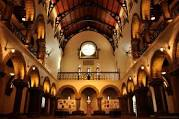
\includegraphics[width =3 in ]{coep}
	
	\vspace{1in}
	\end{figure}
    \item Scenic Beauty
	

	\begin{figure}[H]
	\centering
	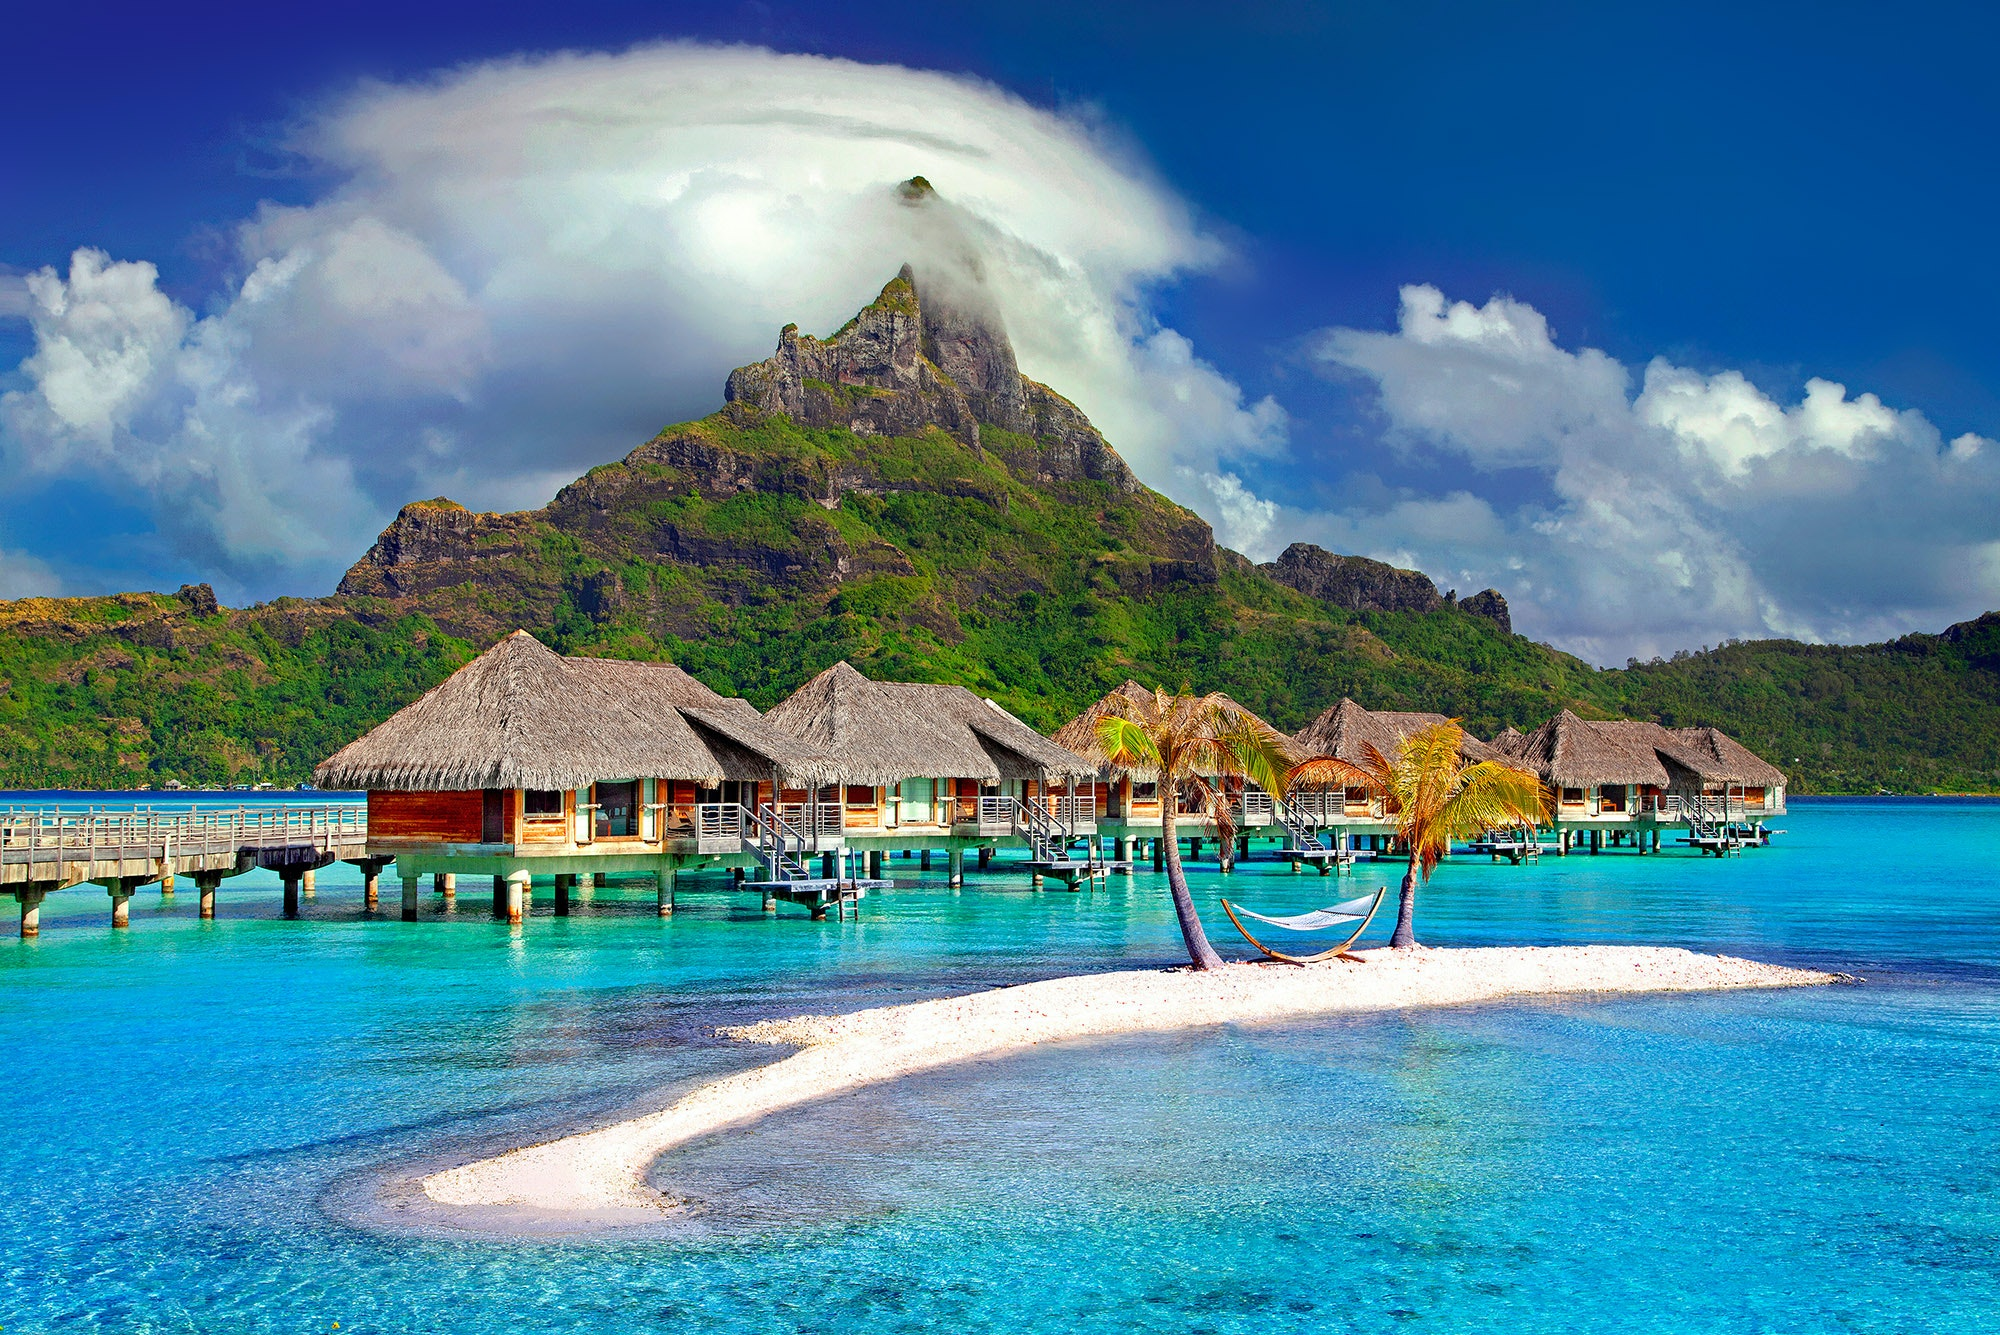
\includegraphics[width =3 in]{image-2}
	
	
	\end{figure}
	
	\item Graphs
	
	\begin{figure}[H]
	\centering
	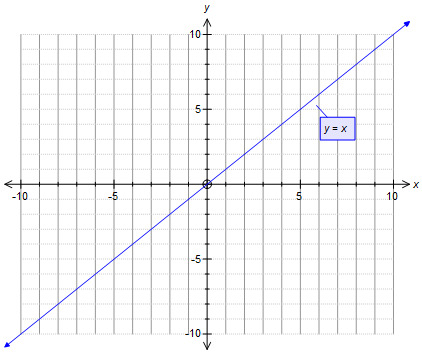
\includegraphics[width = 3 in]{y=xgraph_new}
	\caption{$ y=x$}
	\end{figure}
	\end{enumerate}

\section{Tables}
	\subsection{Countries and its capital}
	The following table shows the Countries and their capitals respectively :\\
	\begin{center}
	
	\begin{tabular}{|c|c|}
	\hline
	\bf Country & \bf CAPITAL \\ \hline
	Qatar & Doha \\ \hline
	India & Delhi \\ \hline
	USA & Washington DC \\ \hline
	Canada & Ottawa \\ \hline
	Mexico & Mexico City \\ \hline
	France & Paris \\ \hline
	Egypt & Cairo \\ \hline
	Scotland	& Edinburgh \\ \hline
	Netherlands	 & Amsterdam \\ \hline
	Portugal & Lisbon \\ \hline
    \end{tabular}
	\end{center}
	
	\pagebreak
\section{Csv To Latex}
	\subsection{Student Data}
	\begin{table}[H]
	\centering
	\csvautotabular[]{student.csv}
	\end{table}
	
	\subsection{Weather Data}
	\begin{table}[H]
	\centering
	\csvautotabular[]{data.csv}
	\end{table}



\pagebreak
\begin{Huge}
\begin{center}
\bf Assignment 4
\end{center}
\end{Huge}



\pagenumbering{gobble}
\maketitle
\clearpage
\pagenumbering{roman}

\section*{Quantum Entanglement}
Quantum entanglement is the phenomenon that occurs when a group of particles are generated, interact, or share spatial proximity in a way such that the quantum state of each particle of the group cannot be described independently of the state of the others, including when the particles are separated by a large distance. The topic of quantum entanglement is at the heart of the disparity between classical and quantum physics: entanglement is a primary feature of quantum mechanics not present in classical mechanics ~\cite{1}. \\
Such phenomena were the subject of a 1935 paper by Albert Einstein, Boris Podolsky, and Nathan Rosen, ~\cite{2} and several papers by Erwin Schrödinger shortly thereafter, ~\cite{3, 4} describing what came to be known as the EPR paradox. Einstein and others considered such behavior impossible, as it violated the local realism view of causality (Einstein referring to it as "spooky action at a distance") ~\cite{5} and argued that the accepted formulation of quantum mechanics must therefore be incomplete. \\
Later, however, the counterintuitive predictions of quantum mechanics were verified ~\cite{6, 7, 8} in tests where polarization or spin of entangled particles was measured at separate locations, statistically violating Bell's inequality. In earlier tests, it could not be ruled out that the result at one point could have been subtly transmitted to the remote point, affecting the outcome at the second location. ~\cite{8} However, so-called "loophole-free" Bell tests have been performed where the locations were sufficiently separated that communications at the speed of light would have taken longer—in one case, 10,000 times longer—than the interval between the measurements.\cite{7, 6}

\clearpage
\begin{thebibliography} {}

\bibitem{1} Overbye, Dennis (10 October 2022). The New York Times. Retrieved 10 October 2022.	
\bibitem{2} Einstein A, Podolsky B, Rosen N; Podolsky; Rosen (1935) Phys. Rev. 47 (10): 777–780. Bibcode:1935PhRv...47..77 Mathematical Proceedings of the Cambridge Philosophical Society. 31 (4): 555–563. Bibcode:1935PCPS...31..555S. doi:10.1017/S0305004100013554. S2CID 121278681.
\bibitem{3} Schrödinger E (1935). "Discussion of probability relations between separated systems". Mathematical Proceedings of the Cambridge Philosophical Society. 31 (4): 555–563. Bibcode:1935PCPS...31..555S. doi:10.1017/S0305004100013554. S2CID 121278681.
\bibitem{4} Schrödinger E. (1936) Mathematical Proceedings of the Cambridge Philosophical Society. 32 (3): 446–452. Bibcode:1936PCPS...32..446S. doi:10.1017/S0305004100019137. S2CID 122822435
\bibitem{5}Speakable and Unspeakable in Quantum Mechanics (PDF). CERN. ISBN 0521334950. Archived from the original (PDF) on 12 April 2015. Retrieved 14 June 2014.
\bibitem{6}Yin, Juan; Cao, Yuan; Yong, Hai-Lin; Ren, Ji-Gang; Liang, Hao; Liao, Sheng-Kai; Zhou, Fei; Liu, Chang; Wu, Yu-Ping; Pan, Ge-Sheng; Li, Li; Liu, Nai-Le; Zhang, Qiang; Peng, Cheng-Zhi; Pan, Jian-Wei (2013). "Bounding the speed of 'spooky action at a distance". Physical Review Letters. 110 (26): 260407.
\bibitem{7} Matson, John (13 August 2012). "Quantum teleportation achieved over record distances". Nature News. doi:10.1038/nature.2012.11163. S2CID 124852641.
\bibitem{8} Francis, Matthew. Quantum entanglement shows that reality can't be local, Ars Technica, 30 October 2012

\end{thebibliography}
\end{document}






















